\documentclass[a4paper]{article}
\usepackage[latin1]{inputenc}
\usepackage[T1]{fontenc}
\usepackage[francais]{babel}
\usepackage{entete}
\usepackage{noitemsep}
\usepackage{euscript} 
\usepackage{amsmath,amssymb,amsfonts,amsthm}
\usepackage{graphicx,graphics,epsfig,subfigure,color}
\usepackage{url}
%\usepackage{algorithm2e}
\usepackage{multicol}
\usepackage{a4wide}
\usepackage{latexsym}
\usepackage{verbatim}
\setlength{\textheight}{23.5cm}
\setlength{\topmargin}{-1cm}
\setlength{\textwidth}{155mm}
\setlength{\oddsidemargin}{2mm}

%\renewcommand{\baselinestretch}{0.85}

%\input{macroAlgo}
%\dontprintsemicolon


\setlength{\parindent}{0pt}  %%suppression indentation


\begin{document}
\selectlanguage{francais}
\author{D. Fourer, L. Lagon}
\newcommand{\universityname}{IUT d'\'Evry-Val-d'Essonne}
\newcommand{\deptname}{D\'epartement TC (S3)}
\newcommand{\years}{2023-2024}

%------------------- TITRE -----------------------------------------
\date{Septembre 2023} 
\TDHead{\universityname}{\deptname}{R3.12, \years}{\large TD3: Calcul et simulations sur un tableur}
%\TDHead{DUT TC}{}{\large TIC3: Fonctions avanc\'ees d'un tableur}
%-------------------------------------------------------------------
\underline{Objectifs:} Analyse et simulations sur tableur

%% calcul iteratif
\exost Deux commerciaux enregistrent chacun un r\'esultat not\'e $x$ et $y$
que nous souhaitons deviner \`a l'aide des indices suivants:
On sait que la diff\'erence entre $x$ et $y$ fait 200 euros, et que le double de $x$ additionn\'e au triple de $y$ fait 4000 euros.\\
En utilisant les \textbf{r\'ef\'erences circulaires}, r\'esolvez le syst\`eme d'\'equations correspondant:
%% https://onedrive.live.com/edit.aspx?resid=1733E4ED310E961!428&app=Excel&wdnd=1&wdPreviousSession=b38af81f%2D833b%2D4091%2Da113%2D904f11263ec4&wdNewAndOpenCt=1541330954971&wdPreviousCorrelation=0e9ce2c2%2D102f%2D4179%2D9aa4%2D74dc2c9b09eb
%------------
\begin{align}
 2 x  + 3 y 	&= 4000\\
 x - y  	&= 200
\end{align}
%------------
%
 \textit{Indications: Utilisez le nommage des cellules contenant $x$ et $y$.
 Affectez la valeur de $x$ et de $y$ apr\`es avoir fait les substitutions n\'ecessaires.\\
 Autorisez ensuite le calcul it\'eratif (Fichier/Options/Formules/Calcul) puis laissez le logiciel de tableur proposer une solution.}
 \begin{center}
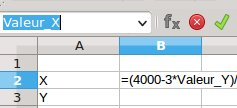
\includegraphics[width=0.25\textwidth]{nommage.jpg}
\end{center}

%% Simulations
%\exost 


%% Gestionnaire de scenarios
\exost Nous souhaitons cr\'eer un simulateur de pr\^et simple et envisager tous les sc\'enarios de remboursement possibles.
\begin{center}
 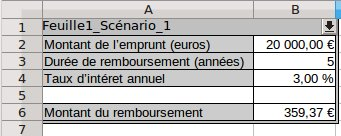
\includegraphics[width=0.5\textwidth]{scenarios.jpg}
\end{center}
\begin{enumerate}
 \item Reproduisez la feuille de calcul ci-dessus. Vous fixerez librement un montant, un taux d'int\'er\^et et une dur\'ee 
 puis vous calculerez le montant des mensualit\'es en utilisant la fonction:\\
 \verb?VPM(Taux_d_interet_annuel/12;Duree_remboursement_en_mois;-Montant_emprunte)?
 \item \`A l'aide du \textbf{gestionnaire de sc\'enarios} (Donn\'ees/Analyse de sc\'enarios), simulez plusieurs sc\'enarios en faisant varier 
 le taux d'int\'er\^et (4\%, 4,5\%, 6\%, 8\%).
 \item Cr\'eez un \textbf{tableau d'hypoth\`eses \`a une entr\'ee} pour les diff\'erents taux d'int\'er\^et.
 \item Cr\'eez un \textbf{tableau d'hypoth\`eses \`a deux entr\'ees} faisant varier la dur\'ee du pr\^et (3 ans, 6 ans, 9 ans et 15 ans).
 \item En raisonnant \`a l'envers, on souhaite d\'eterminer le montant maximum que l'on peut emprunter sachant que
 la capacit\'e de remboursement est de 500 euros/mois. En utilisant \textbf{valeur cible} (Analyse de sc\'enarios / valeur cible),
 recherchez le montant de l'emprunt pour lequel le montant de remboursement (calcul\'e par la fonction \verb?VPM?) est de 500 euros.
\end{enumerate}

\begin{center}
 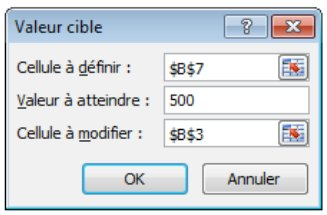
\includegraphics[width=0.25\textwidth]{valeur_cible.jpg}
\end{center}

\end{document}

% End Of File

